% declare our document type
\documentclass[12pt]{extarticle}

%%%%%%%% PACKAGES NEEDED FOR THIS DOCUMENT

% allow us to put pictures in the document
\usepackage{graphicx}
% this line lets us use larger fonts
\usepackage{extsizes}
% this allows us to create ''slides'' in the document
\usepackage[many]{tcolorbox}
% this line lets us caption images inside the ''slides''
% this is neccesary since the slide doesn't allow the use of
% \figure{} inside
\usepackage{caption}
% allows use of courier font
\usepackage{courier}
% make the table of contents links like people are used to
% the hidelinks parts hides link outlines
\usepackage[hidelinks]{hyperref}
% resize the margins
\usepackage[margin=1in]{geometry}
% use utf8 encoding
\usepackage[utf8]{inputenc}
% one of the other packages complained until I put this here
\usepackage[english]{babel}
% allow citations
\usepackage{cite}
% code listings
\usepackage{listings}
% fix single quote in listings
\usepackage{textcomp}

\usepackage[T1]{fontenc}

%%%%%%%%%%% CUSTOM ENVIRONMENT SETUP

% declare a typesetting environment for code/emphasis
\newcommand{\code}[1]{\texttt{\bfseries#1}}
\newenvironment{codeblock}{\bfseries\texttt\bgroup}{\egroup\par}
% better declaration of font environment
%\DeclareTextFontCommand{\codetext}[1]{\code{#1}}
% declare a large font environment for use in the ''slides''
\newcommand{\instruction}[1]{\Large{#1}}
% font environment again
%\DeclareTextFontCommand{\instruction}{\instructionfont}
\newenvironment{instructionblock}{\Large\bgroup}{\egroup}
% declare a ''slide'' text box for use in the document
% the slide is a numbered \section{}
\newtcolorbox[auto counter]{slide}[3][]{%
colback=brown!5!white,colframe=brown!80!gray,height=3.72in,
title={\addcontentsline{toc}{section}{\thetcbcounter ~~ #2}\bf\Large\thetcbcounter ~ #2\hfill #3 \label{slide \thetcbcounter}\setcounter{section}{\thetcbcounter}}}
% declare a ''subslide'' text box for use in the document
% the subslide is a numbered \subsection{}
\newtcolorbox[auto counter,number within=section]{subslide}[3][]{%
colback=brown!5!white,colframe=brown!80!gray,height=3.72in,
title={\addcontentsline{toc}{subsection}{\thetcbcounter ~~ #2}\bf\Large\thetcbcounter ~ #2\hfill #3 \label{slide \thetcbcounter}}}
\renewcommand{\labelitemii}{$\circ$}
\lstset{basicstyle=\ttfamily,keywordstyle=\bfseries\color{blue!80!black},identifierstyle=\bfseries,stringstyle=\color{red},showstringspaces=false,commentstyle=\itshape\color{green!40!black},upquote=true}

% My Environments (keep these)
\newcommand{\ben}{\begin{enumerate}}
\newcommand{\een}{\end{enumerate}}
\newcommand{\bi}{\begin{itemize}}
\newcommand{\ei}{\end{itemize}}
\usepackage{titling}
\newcounter{questionEnumerate}
\usepackage{hyperref}
%%%%%%%%% SET UP OUR TITLE PAGE

\begin{document}
\title{ Vulnerability Scanning }
\author{Nicholas Valenti, Harika Vadapalli, and Ananth Jillepalli}
\date{July 1, 2017 \\ \hyperref[changelog]{Version 1.1}} %\today
\renewcommand{\abstractname}{Executive Summary}
\begin{titlepage}
\maketitle
\pagenumbering{gobble}
\begin{center}

\includegraphics[scale=.5]{UofI}

\large{CS 439/539: Applied Security Concepts}

\vskip 40pt

\end{center}
\begin{abstract}

Vulnerability scanning is often one of the first lines of defense when securing a system. Tools specific to identifying potential attack surfaces can reveal out of date software, services with loose permissions, or other areas of concern. Different tools have different objectives so it's important to be familiar with a variety of ways to analyze your own security capabilities.

\center{\textbf{Prerequisites}}

None.
\end{abstract}


\vfill
\begin{center}
	
\includegraphics[scale=0.5]{cc}
	\vskip 10pt
	This work is licensed under a \href{https://creativecommons.org/licenses/by/4.0/}{Creative Commons Attribution 4.0 International License}.
\end{center}

\end{titlepage}

%%%%%%%%%% TABLE OF CONTENTS

\pagebreak
\tableofcontents

%%%%%%%%%%%%%%%%%%%%%%%%%%%%%%%%%%%%%%%%%%%%%%%%%
%%%%%%    BEGINNING OF ACTUAL DOCUMENT
%%%%%%%%%%%%%%%%%%%%%%%%%%%%%%%%%%%%%%%%%%%%%%%%%

\pagebreak
\pagenumbering{arabic}
\setcounter{section}{1}
\begin{slide}{Objectives}{\hyperref[slide 2]{\textgreater}}
	\vskip 10 pt
	\begin{instructionblock}
		\begin{itemize}
			
\item Understand the importance of vulnerability scanning in protecting a system;
\item Know which tools can be used to perform vulnerability scans;
\item Use vulnerability scans to identify mitigations to attacks.
\end{itemize}
	\end{instructionblock}
\end{slide}
%\vfill

\pagebreak
\begin{slide}{Scanning and Legality}{\hyperref[slide 1]{\textless}\hyperref[slide 3]{\textgreater}}
	\vskip 10 pt
	\begin{instructionblock}
		\begin{itemize}
			\item Like with NMap, scanning a system or network is illegal without permission;
			\item Only perform scans on hardware and software that is isolated and you have written explicit permission from the system owner to scan;
			\item Some tools we will be using, such as metasploit, have even more severe legal implications if they are misused.
		\end{itemize}
	\end{instructionblock}
\end{slide}
%\vfill




\pagebreak
\begin{slide}{Hardware and Software Requirements }{\hyperref[slide 2]{\textless}\hyperref[slide 4]{\textgreater} }
	\begin{instructionblock}
		The tutorial was executed using the following environment:
		\begin{enumerate}
			\item A computer capable of hosting at least 4 virtual machines (VMs);
			\item A virtualization software platform, e.g. VMWare or VirtualBox;
			\item A) Kali VM, B) Ubuntu/Linux VM, C) Windows XP SP2 VM, and D) Windows XP SP3 VM.
		\end{enumerate}
	\end{instructionblock}
\end{slide}

\textbf{Network Diagram:}

\begin{center}
	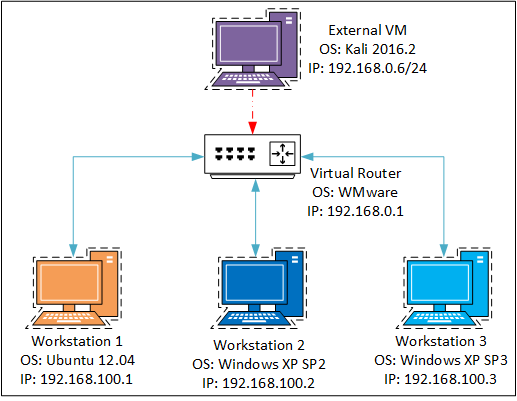
\includegraphics{NetworkDiagram.png}
\end{center}


\pagebreak
\begin{slide}{OpenVAS}{\hyperref[slide 3]{\textless}\hyperref[slide 5]{\textgreater}}
	%\vskip 10 pt
	\begin{instructionblock}
		\begin{itemize}
			\item Open Vulnerability Assessment System;
			\item Free under GNU Public General Public License;
			\item OpenVAS is a framework that includes multiple services and tools to scan for vulnerabilities due to versioning, exploitable software, and more;
			\item Common Vulnerability Scoring System (CVSS).
		\end{itemize}
	\end{instructionblock}
\end{slide}
%\vfill
\begin{enumerate}
	\item OpenVAS split from Nessus, a comparable commercial service, in 2005 when it ceased to be open source.
	\item Nessus still exists and has both a commercial and a limited free Home version.
	\item OpenVAS maintains a free GNU GPL license and is free and was most recently updated with version 8.0 released in April 2015\cite{b3}.
	\item Threats are ranked based on their potential to cause damage but this may differ from their actual impact. Because CVSS ranks threats based on the damage that can be caused if they are successfully exploited some threats may appear that may not pose an actual risk\cite{b1}.
\end{enumerate}
\pagebreak


\begin{slide}{Task 1: OpenVAS\cite{b1}}{\hyperref[slide 4]{\textless}\hyperref[slide 6]{\textgreater}}
	\begin{instructionblock}
		\begin{enumerate}
			\item Set an OpenVAS policy;
			\item Run a scan on a Windows XP SP2 machine;
			\item Research vulnerabilities using built in OpenVAS tools and Internet on BLUE side;
			\item Have information on at least 3 vulnerabilities.
		\end{enumerate}
	\end{instructionblock}
\end{slide}
%\vfill

\begin{enumerate}
	\item OpenVAS will require several pieces of information to create a scan policy including basic identification.
	\item OpenVAS uses a suite of tools to probe a target for information. It is able to detect a number of potential issues and display the results of a scan in an easy to read format.
	\item In order to gain additional information the internet may be used. There are a number of security related websites\cite{b1}.
	\begin{itemize}
		\item http://www.securityfocus.com/;
		\item http://www.packetstormsecurity.org/;
		\item http://www.exploit-db.org/;
		\item http://www.cve.mitre.org/.
	\end{itemize}
	\item Task 1: 5-10 minutes.
\end{enumerate}

%Time: 20 minutes

\pagebreak

\begin{slide}{NMap Scripting Engine (NSE)\cite{b2}}{\hyperref[slide 5]{\textless}\hyperref[slide 7]{\textgreater}}
	\begin{instructionblock}
		\begin{itemize}
			\item NMap has expanded beyond its original scope of simple port scanning and now contains a scripting engine with several publicly available scripts;
			\item Scripts can also be written by users;
			\item Kali stores scripts in \texttt{/usr/share/nmap/scripts};
			\item The \textbf{-sC} flag will tell NMap to run all scripts in the default category in addition to doing a port scan\cite{b1};
			\\
			Additional information can be found with the command \texttt{nmap --script-help <category>}.
		\end{itemize}
	\end{instructionblock}
\end{slide}
%\vfill
Some NSE scripts can harm target systems. While we will not be using them there are entire sections dedicated to malware, DDOS, and other exploitation. It is important to use the help functions before running any NSE scripts in order to determine whether or not they're dangerous\cite{b2}.

\pagebreak

\begin{slide}{Challenge 1: NSE}{\hyperref[slide 6]{\textless}\hyperref[slide 8]{\textgreater}}
	\vskip 10 pt
	\begin{instructionblock}
		\begin{enumerate}
			\item Use the NMap Scripting Engine to run a script scan on all found machines;
			\item Get information on the ftp-anon script from NMap's help function;
			\item Use NSE to run only the ftp-anon script.
		\end{enumerate}
	\end{instructionblock}
\end{slide}
%\vfill
\begin{enumerate}
	\item Vulnerable machines might be found on a different subnet.
	\item We already know that the \textbf{-sC} flag will run all default scripts. How can we run scripts in other categories?
	\item Try using the built in help in order to discover how NSE handles single script execution. What other scripts can you find that get you results? Research using the Internet if you get stuck.
	\item Deliverable: What does this script look for and are there any machines that are susceptible.
\end{enumerate}

\pagebreak

\begin{slide}{Metasploit\cite{b4}}{\hyperref[slide 7]{\textless}\hyperref[slide 9]{\textgreater}}
	\vskip 10 pt
	\begin{instructionblock}
		\begin{itemize}
			\item The Metasploit Framework is a widely used penetration testing framework;
			\item Metasploit can be used to quickly assess the actual impact of a found vulnerability;
			\item Public exploits can be modified in order to work in your environment;
			\item Always be vigilant, not all public exploit code works as advertised. 
		\end{itemize}
	\end{instructionblock}
\end{slide}
%\vfill
\begin{enumerate}
	\item There is both an open source version and a commercial version owned by Rapid7\cite{b4}.
	\item Many of the same websites as listed in the NMap portion of this tutorial can be used to research exploits\cite{b1}.
\end{enumerate}


\pagebreak

\begin{slide}{Task 2: Starting Metasploit\cite{b1}}{\hyperref[slide 8]{\textless}\hyperref[slide 10]{\textgreater}}
	\vskip 10 pt
	\begin{instructionblock}
		The Metasploit console can be started using these commands:\\
		
			root@kali:$\sim$\# \textbf{service postgresql start};
			
            root@kali:$\sim$\# \textbf{service metasploit start};
            
			root@kali:$\sim$\# \textbf{msfconsole}.
			
	\end{instructionblock}
\end{slide}
%\vfill
\begin{enumerate}
	\item PostgreSQL is used by Metasploit to keep track of your actions.
	\item msfcli is a command line interface that can also be used to interact with metasploit without having to run the Metasploit console directly. We won't be using it in this tutorial.
	\item In a GUI based system Metasploit will be listed under programs and can be launched this way as well, but will open the same console.
\end{enumerate}


\pagebreak

\begin{slide}{Challenge 2: Find information on the MS08-67 patch}{\hyperref[slide 9]{\textless}\hyperref[slide 11]{\textgreater}}
	\vskip 10 pt
	\begin{instructionblock}
		\begin{enumerate}
			\item Use Metasploit's built in search function on RED;
			\item Feel free to use the Internet on BLUE as well;
			\item What is the issues that the MS08-67 patch resolved?
			\item What platforms is it used on and how was it fixed?
		\end{enumerate}
	\end{instructionblock}
\end{slide}
%\vfill

\begin{enumerate}
	\item MS08-067 was a patch that fixed the ms08\_067\_netapi vulnerability in 2008 (hence ms08) \cite{b6}.
	\item The vulnerability is commonly known and affects many Windows XP machines today, affecting a flaw in the NetAPI32.dll file.
	\item We can scan for out of date patches or the signs of out of date services using OpenVAS, NMap, or even metasploit. Usually scanning is done when there is a suspected vulnerability and we can use our results to find out what is and isn't up to date. Remember the number one mitigation against known vulnerabilities such as the public Metasploit database is patching your software.
	\item Deliverable: a report on the MS08-67 patch and the exploit it addressed, class discussion as information is discovered.
	\item Time 5-10 minutes.
\end{enumerate}

% 40 minutes

\pagebreak
\begin{slide}{Metasploit Scanning\cite{b1}}{\hyperref[slide 10]{\textless}\hyperref[slide 12]{\textgreater}}
	%\vskip 10 pt
	\begin{instructionblock}
		\begin{enumerate} 
			\item Similarly to NMap, Metasploit has evolved beyond its original design and now incorporates vulnerability assessment;
			\item Metasploit Scanner Modules allow us to identify vulnerabilities that might be exploited during an attack. 
		\end{enumerate}
	\end{instructionblock}
\end{slide}
%\vfill


\pagebreak
\begin{slide}{Questions I}{\hyperref[slide 11]{\textless}\hyperref[slide 13]{\textgreater}}
	\begin{instructionblock}
		\begin{enumerate}
			\item What are three tools that can be used for vulnerability scanning?
			\item How can vulnerability scanning used to secure a system?
		\end{enumerate}
	\end{instructionblock}
\end{slide}
%\vfill
\begin{itemize}
	\item Many examples of tools are found throughout the tutorial.
	\item What is an attack surface? What resources do we have beyond the ones available in Kali?
	\begin{enumerate}
		\item OpenVAS/Nessus, NMap, Nikto, Metasploit, XAMPP, etc;
		\item Identifying an attack surface, finding old versions of software, find neglected ports, etc.
	\end{enumerate}
\end{itemize}
\pagebreak

\begin{slide}{Task 3: Metasploit Modules}{\hyperref[slide 12]{\textless}\hyperref[slide 14]{\textgreater}}
\begin{instructionblock}
\begin{enumerate}
		\item Metasploit comes with many modules that can be used to do everything from scan to actual delivery of payloads;
		\item We can use a scanner module to gain information about a target\cite{b4};\\
		
		msf > \textbf{use scanner/ftp/anonymous};
		
		\item Use \textbf{show options} to find more information about your current module;
\end{enumerate}
\end{instructionblock}
\end{slide}
%\vfill
\begin{itemize}
	\item When loading a module (such as \textbf{scanner/ftp/anonymous}) the msf command line changes to reflect which module is currently in use\cite{b4};
	\item The \textbf{show options} command will show targets, ports, and more information that we will go over in more detail in the next slide.
\end{itemize}
\pagebreak

\begin{slide}{Metasploit Modules\cite{b1}}{\hyperref[slide 13]{\textless}\hyperref[slide 15]{\textgreater}}
	\begin{instructionblock}
			Metasploit Options:
		\begin{itemize}			
			\item RHOST;
			\item RPORT;
			\item SMBPIPE;
			\item Exploit Target.
		\end{itemize}
	\end{instructionblock}
\end{slide}
%vfill
\begin{itemize}
	\item RHOST is the remote host Metasploit is targeting.
	\item RPORT is the port we are targeting and can be set manually. In our case if there is a default port that the currently loaded module uses it will be set automatically.
	\item SMBPIPE is out of the scope of this tutorial but is essentially the medium we are communicating across on the network.
	\item Exploit Target details the specific operating system and version we are targeting. By using the \textbf{show targets} command we can see what the possibly vulnerable targets for our current exploit can be. Automatic targeting will attempt to fingerprint the target and select an appropriate payload if it can.
\end{itemize}

\pagebreak
\begin{slide}{Challenge 3: Metasploit Scanning}{\hyperref[slide 14]{\textless}\hyperref[slide 16]{\textgreater}}
\vskip 5pt
\begin{instructionblock}
	\begin{enumerate}
	\item Use the \textbf{scanner/ftp/anonymous} module to scan machines on your local network;
	\item How many systems can you find that allow anonymous FTP?
	\item Use Internet on BLUE to find other scanning modules that could be used;
	\item When you're satisfied change your module to the ms08\_067\_netapi exploit we researched earlier.
	\end{enumerate}
\end{instructionblock}
\end{slide}


\begin{enumerate}
	\item Use NMap to find potential targets on your network.
	\item How much additional information can you find about these systems in an unobtrusive way?
	\item The module we used earlier is pathed at \textbf{windows/smb/ms08\_067\_netapi}. How do you change your active Metasploit module?
	\item Deliverable: a brief report with any found systems that have open FTP (we found this earlier using NSE so this challenge should be brief), class discussion about other scanning modules.
	\item Time: 5-10 minutes.
\end{enumerate}
%Time 75 minutes
\pagebreak

\begin{slide}{More Metasploit Scanning\cite{b1}}{\hyperref[slide 15]{\textless}\hyperref[slide 17]{\textgreater}}
\vskip 5pt
\begin{instructionblock}
\begin{itemize}
	\item Metasploit can be used to connect to a target to see if it's vulnerable without actually delivering a payload;
	\item Set RHOST to the IP address of the Windows XP SP2 machine and make sure the proper module is set;
	\item Use the \textbf{check} command to probe the specified target;
	\item Check only works on some supported modules.
\end{itemize}
\end{instructionblock}
\end{slide}
%\vfill


\pagebreak
\begin{slide}{Task 5: Metaspoit Payload Delivery}{\hyperref[slide 16]{\textless}\hyperref[slide 18]{\textgreater}}
\vskip 5pt
\begin{instructionblock}
	\begin{itemize}
		\item Post-scanning of our Windows XP SP2 target, lets take a moment to see just how vulnerable an unpatched system is;
		\item Make sure RHOST is set correctly and the proper module is loaded into Metasploit;
		\item A list of compatible payloads can be found by using the \textbf{show payloads} command.
	\end{itemize}
\end{instructionblock}
\end{slide}
%\vfill

\pagebreak
\begin{slide}{Task 5 (Cont): Metasploit Payload Delivery}{\hyperref[slide 17]{\textless}\hyperref[slide 19]{\textgreater}}
	\vskip 5pt
	\begin{instructionblock}
	\begin{itemize}
			\item Use the \textbf{exploit} command to launch the payload once you're happy with the settings;
			\item Observe and make a note of subsequent happenings.
		\end{itemize}
	\end{instructionblock}
\end{slide}
%\vfill
\begin{enumerate}
	\item Gaining root access or setting up reverse shells is usually a somewhat labor intensive process;
	\item This is not even the easiest way to exploit a vulnerable system.
\end{enumerate}


\pagebreak
\begin{slide}{Challenge 4: Windows XP SP3}{\hyperref[slide 18]{\textless}\hyperref[slide 20]{\textgreater}}
\vskip 5pt
\begin{instructionblock}
	\begin{enumerate}

	\item One of the biggest tools in our defensive arsenal is patching;
	\item Find the Windows XP SP3 machine on your network and scan it using all the tools you have so far;
	\item How many vulnerability differences can you find between the two? (Note that they are both largely unpatched);
	\item BE CAREFUL not to push a payload on this machine, it can cause damage and will probably be noticed. Remember you want to defend your network, not destroy it!

	\end{enumerate}
\end{instructionblock}
\end{slide}
\begin{itemize}
	\item Time: up to 15-20 minutes as available;
	\item There are a lot of vulnerabilities on both machines, it might take time to find differences;
	\item Deliverables: a list of any found vulnerabilities.
\end{itemize}
%\vfill

%Time: at most 90 minutes

\pagebreak
\begin{slide}{Nikto\cite{b7}}{\hyperref[slide 19]{\textless}\hyperref[slide 21]{\textgreater}}
	\vskip 5pt
	\begin{instructionblock}
		\begin{enumerate}
			
			\item Nikto is like OpenVAS for network services;
			\item Checks for dangerous files, outdated versions of services, server options, etc.;
			\item In order to run a scan use \textbf{nikto -h <IP Address>};
			\item Full feature list can be found at http://cirt.net/Nikto2.
			
		\end{enumerate}
	\end{instructionblock}
\end{slide}
%\vfill

\pagebreak
\begin{slide}{Challenge 5: Nikto}{\hyperref[slide 20]{\textless}\hyperref[slide 22]{\textgreater}}
	\vskip 5pt
	\begin{instructionblock}
		\begin{enumerate}
			
			\item There is a metasploitable Ubuntu machine located on your local RED network;
			\item If you haven't already found it do so now and run a Nikto scan on it (RED side);
			\item Research some of the potential issues Nikto discovered:
			\begin{itemize}
				\item Research can be done on the Internet.
			\end{itemize}
			
		\end{enumerate}
	\end{instructionblock}
\end{slide}
%\vfill

\begin{itemize}
	\item Time: 5-10 minutes. 
\end{itemize}

%Time: 90 minutes

\pagebreak
\begin{slide}{Challenge 6: Mitigations\cite{b1}}{\hyperref[slide 21]{\textless}\hyperref[slide 23]{\textgreater}}
\vskip 5pt
\begin{instructionblock}
	\begin{enumerate}
	\item There is a metasploitable linux machine located on your local network;
	\item Use everything you've learned to identify and close as many attack surfaces as you can;
	\item Assume the owner of the metasploitable machine wants to keep FTP, HTTPS, and IRC open.
	\end{enumerate}

\end{instructionblock}
\end{slide}
%\vfill
\begin{itemize}
	\item What services are required? How do you handle services that might be vulnerable but are required for business or personal purposes?
	\item Feel free to use material from previous tutorials such as firewalls to assist you in your efforts.
	\item Time: 30+ minutes.
\end{itemize}

\pagebreak
\begin{slide}{Bonus Slide: Armitage\cite{b5}}{\hyperref[slide 22]{\textless}\hyperref[slide 24]{\textgreater}}
	\vskip 5pt
	\begin{instructionblock}
		\begin{itemize}
			\item Armitage is a utility suite built around NMap, Metasploit, and other tools to provide easy access to the functions of all programs under its umbrella.
			\item It is capable of sharing logs and information between team members as well as making exploit suggestions, and remembers details about systems found from any platform.
			\item Check out http://www.fastandeasyhacking.com/manual, for more information on Red Team Operations.
		\end{itemize}
		
	\end{instructionblock}
\end{slide}
\vfill
\pagebreak

\begin{slide}{Conclusion}{\hyperref[slide 23]{\textless}}
	\vskip 5pt
	\begin{instructionblock}
		\begin{itemize}
		\item Vulnerability scanning is an important tool in any security professional arsenal;
		\item Keeping your tools and services up to date and understanding what is going on with your network and ports.
	    \end{itemize}
	\end{instructionblock}
\end{slide}
%\vfill
\vfill
A significant source for this tutorial is: \cite{b1}

\pagebreak
\phantomsection
\textbf{Changelog:}
\label{changelog}
\vspace{6mm}


\begin{tabular}{ |p{1cm}|p{3cm}|p{3cm}|p{5cm}|  }
\hline
\multicolumn{4}{|c|}{Vulnerability Scanning} \\
\hline
\texttt{Ver.} & \texttt{Date} & \texttt{Authors} & \texttt{Changes} \\
\hline
v1 & Feb 13th 2017 & Nicholas Valenti and Harika Vadapalli & Initial Tutorial. \\
\hline
v1.1 & July 1st 2017 & Ananth Jillepalli & Standardization (network layout diagram, edits, consistency, TeX markup cleaning, and more). \\ \hline
\end{tabular}

% bibliography on last page
\pagebreak
% this style of bibliography shows urls
\bibliographystyle{IEEEtran}

\begin{thebibliography}{9}

\bibitem{b1}
Weidman, Georgia, "Penetration Testing: A Hands-On Introduction to Hacking", No Starch Press. San Francisco, CA, 2014.

\bibitem{b2}
Gordon Lyon, Charles McFarland, "NMap Scripting Engine (NSE)", Insecure.org.
\url{https://nmap.org/book/man-nse.html}

\bibitem{b3}
N.A., "About OpenVAS Software", Systems Characteristics Producer
\url{http://www.openvas.org/software.html}

\bibitem{b4}
ckirsch, "What is Penetration Testing", Rapid7,
\url{https://community.rapid7.com/docs/DOC-2248}

\bibitem{b5}
N.A., "Fast and Easy Hacking", Strategic Cyber LLC.
\url{http://www.fastandeasyhacking.com/manual}

\bibitem{b6}
N.A., "Microsoft Security Bulletin MS08-067 - Critical", Microsoft.
\url{https://technet.microsoft.com/en-us/library/security/ms08-067.aspx}

\bibitem{b7}
Chris Sullo and David Lodge, "Nikto2", CIRT.net.
\url{https://cirt.net/Nikto2}

%example biblio entry
\iffalse
\bibitem{Winkler15}
    Winkler, I.
    2015
    \textit{The 'Sophisticated Attack' Myth}\\
    ComputerWorld, The Internet, 2015.
\fi 

%1 book
%2 NSE
%3 OpenVAS
%4 Metasploit
%5 Armitage

\end{thebibliography}


\end{document}